\documentclass[twocolumn,prl]{revtex4-1}
% \documentclass{article}
\usepackage{amsmath}
\usepackage{graphicx}
\usepackage{stfloats}

\begin{document}
\title{Capillary Forces Between Corners}
\author{Student A}
\author{Student B}
\author{Student C}
\author{Professor}
\affiliation{Brown University}

\begin{abstract}
% \lipsum
	Lorem ipsum dolor sit amet, consectetur adipisicing elit, sed do eiusmod tempor incididunt ut labore et dolore magna aliqua. Ut enim ad minim veniam, quis nostrud exercitation ullamco laboris nisi ut aliquip ex ea commodo consequat. Duis aute irure dolor in reprehenderit in voluptate velit esse cillum dolore eu fugiat nulla pariatur. Excepteur sint occaecat cupidatat non proident, sunt in culpa qui officia deserunt mollit anim id est laborum.
\end{abstract}

\maketitle

	Nearby floating objects mutually attract through capillary interactions in a shape-dependent mechanism. 
	
	These capillary interactions, commonly known as the Cheerios effect, is a gravity and surface-wetting driven process communicated along the interface. This attraction has been observed or postulated in locomotion of aquatic plant seeds\cite{peruzzo2013capillary}, meniscus climbing insects\cite{hu2005meniscus} and directed colloidal self-assembly\cite{fan2004assembly}. Thus far, studies have extensively focused on either smooth objects//cite//, objects spaced far apart//cite// or on objects on an initially curved interface//cite//. There  
	
	
	//Planar Contact line//
	//Objects may become non-planar//
	
	
	Figure 1 presents qualitative observations of the attraction between two floating 1'' wide acrylic triangles as they approach each other, viewed from above. For a large class of relative initial positions and orientations, they rotate such that corners kiss first, after which they will fold or slide into a more stable final configuration. Prior to kissing, it appears that attraction is localized at the corners where there is a curvature singularity //cite//. To the best of our knowledge, the force of attraction between sharp objects of comparable sizes have never been quantified before
	
	and that the attractive behavior of sharp objects is different from smooth objects. The force of attraction due to corners have never been quantified before. In this letter, we show that the attraction scales as $d^{14/5}$, where $d$ is the distance between 60 $^{\circ} $ corners. 
	
	The process described above depends entirely on the shape of the meniscus around each object. We calculate using 


//Show experimental set-up//
\begin{figure*}[htb!]

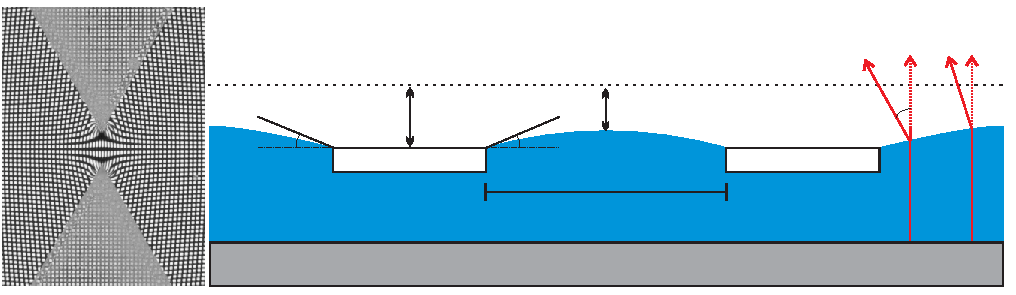
\includegraphics{Figures/Fig2.pdf}
\caption{Lorem ipsum dolor sit amet, consectetur adipisicing elit, sed do eiusmod tempor incididunt ut labore et dolore magna aliqua. Ut enim ad minim veniam, quis nostrud exercitation ullamco laboris nisi ut aliquip ex ea commodo consequat.}
\end{figure*}


\begin{equation}\label{eqn:forcebalance}
F \approx \frac{\sigma}{2} \int _C [(\frac{u^2}{l_c^2}- u_n^2 +u_t^2 )d\textbf{t} - 2u_n u_t d\textbf{n}]
\end{equation}
	the attractive force, $F$, by applying a force balance on a loop enclosing the meniscus\cite{he2013capillary}. u is the vertical displacement ... u/lc is the hydrostatic term and the gradients are the ...



//As a check, show attractive force between spheres and compare with literature//

Force from deformation of meniscus. Measure Meniscus deformations - Verify using circles. Use for triangles for d ~ lc and $d << lc$.

\section{Results}
//Show derivation for conformal mapping on angles//

//Show ux scaling for the inner and outer region//

//Show Force plot and regions of scaling//

\section{Discussion}
What does this mean?

Force concentrated at vertices is much stronger than force between smooth edges.

\section{Figures}
Figure 1: Analog of introduction in figures

Figure 2: Schematic for experiment and representative results 

Figure 3: Power law scaling and force vs. distances.

Figure 4: On the boundary integral methods

\section{notes}


\bibliographystyle{plain}
\bibliography{article}
\end{document}
